\documentclass[aspectratio=43]{beamer}
% \documentclass[aspectratio=169]{beamer}

% Title --------------------------------------------
\title[Lecture 1: Introduction to Research Design]{\Large Introduction to Research Design}
\author[]{Francisco Villamil}
\date[]{Research Design for Social Sciences\\MA Computational Social Science, UC3M\\Fall 2023}

%%% NOTE -- CHECK THIS: https://github.com/paulgp/beamer-tips


%%% Building heavily on https://github.com/kylebutts/templates

% xcolor, define them
\usepackage{xcolor}

% TEXT COLORS
\definecolor{red}{HTML}{9a2515}
\definecolor{yellow}{HTML}{EBC944}
\definecolor{asher}{HTML}{555F61}
\definecolor{jet}{HTML}{131516}

% THEME COLORS
\definecolor{accent}{HTML}{107895}
\definecolor{accent2}{HTML}{9a2515}

% Color commands
\newcommand\red[1]{{\color{red}#1}}
\newcommand\yellow[1]{{\color{yellow}#1}}
\newcommand\asher[1]{{\color{asher}#1}}

\newcommand\BGred[1]{{\colorbox{red!80!white}{#1}}}
\newcommand\BGyellow[1]{{\colorbox{yellow!80!white}{#1}}}
\newcommand\BGasher[1]{{\colorbox{asher!80!white}{#1}}}

% Appendix numbering
\usepackage{appendixnumberbeamer}

% Beamer Options -------------------------------------

% Background
\setbeamercolor{background canvas}{bg = white}

% Change text margins
\setbeamersize{text margin left = 25pt, text margin right = 15pt}

% \alert
\setbeamercolor{alerted text}{fg = accent2}

% Frame title
\setbeamercolor{frametitle}{bg = white, fg = jet}
\setbeamercolor{framesubtitle}{bg = white, fg = accent}
\setbeamerfont{framesubtitle}{size = \small, shape = \itshape}

% Block
\setbeamercolor{block title}{fg = white, bg = accent2}
\setbeamercolor{block body}{fg = jet, bg = jet!10!white}

% Title page
\setbeamercolor{title}{fg = jet}
\setbeamercolor{subtitle}{fg = accent}

%% Custom \maketitle and \titlepage
\setbeamertemplate{title page}
{
    \begin{centering}
      % \vspace{20mm}
      {\Large \usebeamerfont{title}\usebeamercolor[fg]{title}\inserttitle}\\ \vskip0.25em%
      \ifx\insertsubtitle\@empty%
      \else%
        {\usebeamerfont{subtitle}\usebeamercolor[fg]{subtitle}\insertsubtitle\par}%
      \fi%
      {\vspace{10mm}\insertauthor}\\
      \ifx\insertinstitute\@empty%
      \else%
        {\vspace{5mm}\color{asher}\scriptsize{\insertinstitute}}\\\vspace{5mm}
      \fi%
      {\color{asher}\small{\insertdate}}\\
    \end{centering}
}

% Table of Contents
\setbeamercolor{section in toc}{fg = accent!70!jet}
\setbeamercolor{subsection in toc}{fg = jet}

% Button
\setbeamercolor{button}{bg = accent}

% Remove navigation symbols
\setbeamertemplate{navigation symbols}{}

% Table and Figure captions
\setbeamercolor{caption}{fg=jet!70!white}
\setbeamercolor{caption name}{fg=jet}
\setbeamerfont{caption name}{shape = \itshape}

% Put slide number / total slides at the bottom right
\makeatother
\makeatletter
\setbeamertemplate{footline} %{\hfill\insertframenumber/\inserttotalframenumber}
{%
  \leavevmode%
  \hbox{
  \begin{beamercolorbox}[wd=\paperwidth,ht=2.5ex,dp=1.125ex,leftskip=.3cm,rightskip=.3cm plus1fil]{footlinecolor}%
    \color{asher}{{\let\hyperlink\@secondoftwo\insertshorttitle}\hfill\insertshortauthor\hfill\insertshortdate\hfill\insertframenumber/\inserttotalframenumber}
  \end{beamercolorbox}}%
  \vskip0pt%
}
\makeatother
\makeatletter

% Bullet points

%% Fix left-margins
\settowidth{\leftmargini}{\usebeamertemplate{itemize item}}
\addtolength{\leftmargini}{\labelsep}

%% enumerate item color
\setbeamercolor{enumerate item}{fg = accent}
\setbeamerfont{enumerate item}{size = \small}
\setbeamertemplate{enumerate item}{\insertenumlabel.}

%% itemize
\setbeamercolor{itemize item}{fg = accent!70!white}
\setbeamerfont{itemize item}{size = \small}
\setbeamertemplate{itemize item}[circle]
\setlength{\itemsep}{0pt plus 6pt}

%% right arrow for subitems
\setbeamercolor{itemize subitem}{fg = accent!60!white}
\setbeamerfont{itemize subitem}{size = \small}
\setbeamertemplate{itemize subitem}{$\rightarrow$}

\setbeamertemplate{itemize subsubitem}[square]
\setbeamercolor{itemize subsubitem}{fg = jet}
\setbeamerfont{itemize subsubitem}{size = \small}

% References

%% Bibliography Font, roughly matching aea
\setbeamerfont{bibliography item}{size = \footnotesize}
\setbeamerfont{bibliography entry author}{size = \footnotesize, series = \bfseries}
\setbeamerfont{bibliography entry title}{size = \footnotesize}
\setbeamerfont{bibliography entry location}{size = \footnotesize, shape = \itshape}
\setbeamerfont{bibliography entry note}{size = \footnotesize}

\setbeamercolor{bibliography item}{fg = jet}
\setbeamercolor{bibliography entry author}{fg = accent!60!jet}
\setbeamercolor{bibliography entry title}{fg = jet}
\setbeamercolor{bibliography entry location}{fg = jet}
\setbeamercolor{bibliography entry note}{fg = jet}

%% Remove bibliography symbol in slides
\setbeamertemplate{bibliography item}{}





% Links ----------------------------------------------

\usepackage{hyperref}
\hypersetup{
  colorlinks = true,
  linkcolor = accent2,
  filecolor = accent2,
  urlcolor = accent2,
  citecolor = accent2,
}


% Line spacing --------------------------------------
\usepackage{setspace}
\setstretch{1.2}


% \begin{columns} -----------------------------------
\usepackage{multicol}


% % Fonts ---------------------------------------------
% % Beamer Option to use custom fonts
% \usefonttheme{professionalfonts}
%
% % \usepackage[utopia, smallerops, varg]{newtxmath}
% % \usepackage{utopia}
% \usepackage[sfdefault,light]{roboto}
%
% % Small adjustments to text kerning
% \usepackage{microtype}



% Remove annoying over-full box warnings -----------
\vfuzz2pt
\hfuzz2pt


% Table of Contents with Sections
\setbeamerfont{myTOC}{series=\bfseries, size=\Large}
\AtBeginSection[]{
        \frame{
            \frametitle{Roadmap}
            \tableofcontents[current]
        }
    }


% References ----------------------------------------
\usepackage[
    citestyle= authoryear,
    style = authoryear,
    natbib = true,
    backend = biber
]{biblatex}

% Smaller font-size for references
\renewcommand*{\bibfont}{\small}

% Remove "In:"
\renewbibmacro{in:}{}

% Color citations for slides
\newenvironment{citecolor}
    {\footnotesize\begin{color}{accent2}}
    {\end{color}}

\newcommand{\citetcolor}[1]{{\footnotesize\textcolor{asher}{\citet{#1}}}}
\newcommand{\citepcolor}[1]{{\footnotesize\textcolor{asher}{\citep{#1}}}}

% Tables -------------------------------------------
% Tables too big
% \begin{adjustbox}{width = 1.2\textwidth, center}
\usepackage{adjustbox}
\usepackage{array}
\usepackage{threeparttable, booktabs, adjustbox}

% Fix \input with tables
% \input fails when \\ is at end of external .tex file

\makeatletter
\let\input\@@input
\makeatother

% Tables too narrow
% \begin{tabularx}{\linewidth}{cols}
% col-types: X - center, L - left, R -right
% Relative scale: >{\hsize=.8\hsize}X/L/R
\usepackage{tabularx}
\newcolumntype{L}{>{\raggedright\arraybackslash}X}
\newcolumntype{R}{>{\raggedleft\arraybackslash}X}
\newcolumntype{C}{>{\centering\arraybackslash}X}

% Figures

% \imageframe{img_name} -----------------------------
% from https://github.com/mattjetwell/cousteau
\newcommand{\imageframe}[1]{%
    \begin{frame}[plain]
        \begin{tikzpicture}[remember picture, overlay]
            \node[at = (current page.center), xshift = 0cm] (cover) {%
                \includegraphics[keepaspectratio, width=\paperwidth, height=\paperheight]{#1}
            };
        \end{tikzpicture}
    \end{frame}%
}

% subfigures
\usepackage{subfigure}


% Highlight slide -----------------------------------
% \begin{transitionframe} Text \end{transitionframe}
% from paulgp's beamer tips
\newenvironment{transitionframe}{
    \setbeamercolor{background canvas}{bg=accent!60!black}
    \begin{frame}\color{accent!10!white}\LARGE\centering
}{
    \end{frame}
}


% Table Highlighting --------------------------------
% Create top-left and bottom-right markets in tabular cells with a unique matching id and these commands will outline those cells
\usepackage[beamer,customcolors]{hf-tikz}
\usetikzlibrary{calc}
\usetikzlibrary{fit,shapes.misc}

% To set the hypothesis highlighting boxes red.
\newcommand\marktopleft[1]{%
    \tikz[overlay,remember picture]
        \node (marker-#1-a) at (0,1.5ex) {};%
}
\newcommand\markbottomright[1]{%
    \tikz[overlay,remember picture]
        \node (marker-#1-b) at (0,0) {};%
    \tikz[accent!80!jet, ultra thick, overlay, remember picture, inner sep=4pt]
        \node[draw, rectangle, fit=(marker-#1-a.center) (marker-#1-b.center)] {};%
}


\begin{document}
% ====================================================

% ----------------------------------------------------
\begin{frame}

  \titlepage

\end{frame}
% ----------------------------------------------------

% ----------------------------------------------------
\begin{frame}
\frametitle{A real example}
\centering

\begin{itemize}
  \item Racing team deciding whether to race or not in the last session
  \item Car engine has blown out in 7 out of 24 past races
  \begin{itemize}
    \item Should we risk an explosion and go bankrupt or race?
  \end{itemize}
  \item A mechanic has a last-minute gut feeling that it might have to do with temperature
  \item Forecast for race: very cold day
\end{itemize}

\end{frame}
% ----------------------------------------------------

% ----------------------------------------------------
\imageframe{../img/challenger1}
% ----------------------------------------------------

% ----------------------------------------------------
\imageframe{../img/challenger2}
% ----------------------------------------------------

% ----------------------------------------------------
\imageframe{../img/challenger_wiki}
% ----------------------------------------------------

% ----------------------------------------------------
\begin{frame}
\frametitle{Introduction}
\centering

\begin{itemize}
  \item<1-> What is this course about?
  \item<1-> Expectations?
  \item[]<2->
  \item<2-> \textbf{What is research? And why do we need to design it?}
\end{itemize}

\end{frame}
% ----------------------------------------------------

% ----------------------------------------------------
\begin{frame}
\frametitle{Types of research}
\centering

\begin{itemize}
  \item \textit{Theoretical} and \textit{empirical} research
  \item \textit{Qualitative} and \textit{quantitative} empirical research
\end{itemize}

\end{frame}
% ----------------------------------------------------

% ----------------------------------------------------
\begin{frame}
\frametitle{Empirical Research}
\centering

\begin{itemize}
  \item Goal: answer a question using empirical evidence
  \item How? exploiting \textbf{empirical variation}
  \item Research design is essentially knowing which variation to look at, how to measure it, how to analyze it, how to interpret it, etc -- it's about inference
\end{itemize}

\end{frame}
% ----------------------------------------------------

% ----------------------------------------------------
\begin{frame}
\frametitle{Empirical evidence and claims}
\centering

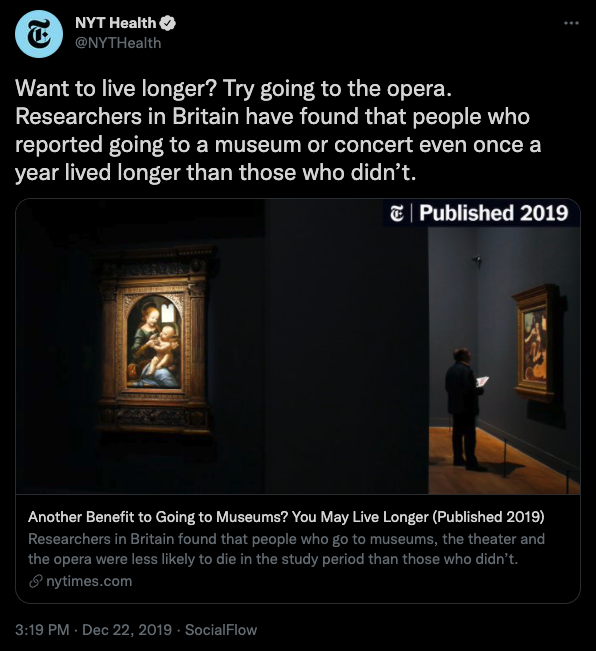
\includegraphics[width = 0.65\textwidth]{../img/nyt_museums}

\end{frame}
% ----------------------------------------------------

% ----------------------------------------------------
\imageframe{../img/psycho1}
% ----------------------------------------------------

% ----------------------------------------------------
\imageframe{../img/psycho2}
% ----------------------------------------------------

% ----------------------------------------------------
\imageframe{../img/psycho3}
% ----------------------------------------------------

% ----------------------------------------------------
\begin{frame}
\frametitle{Opinions about claims?}
\centering

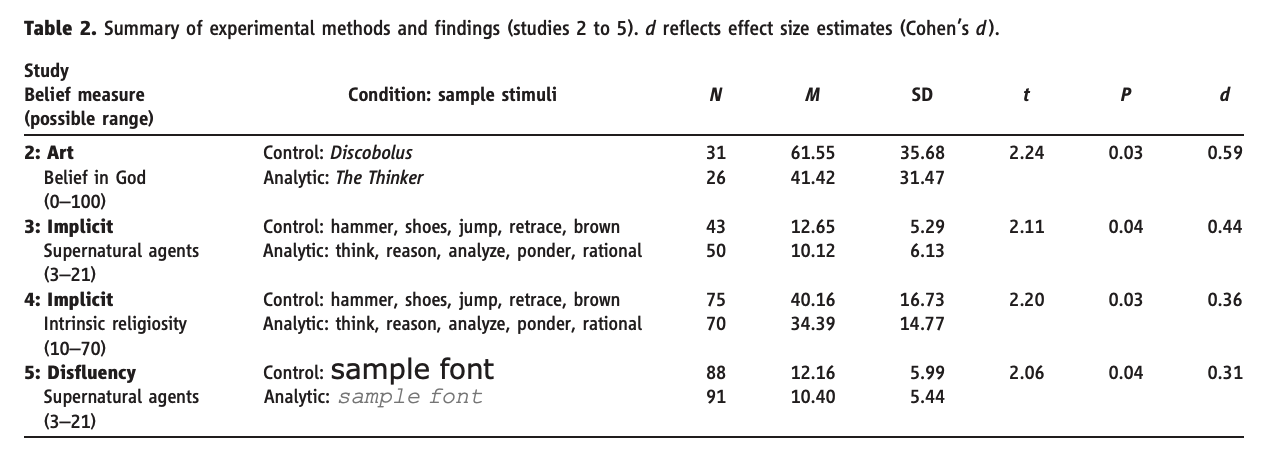
\includegraphics[width = \textwidth]{../img/psycho4}

\end{frame}
% ----------------------------------------------------

% ----------------------------------------------------
\imageframe{../img/replicationcrisis1}
% ----------------------------------------------------

% ----------------------------------------------------
\imageframe{../img/replicationcrisis2}
% ----------------------------------------------------

% ----------------------------------------------------
\imageframe{../img/derecho2022a}
% ----------------------------------------------------

% ----------------------------------------------------
\imageframe{../img/derecho2022b}
% ----------------------------------------------------

% ----------------------------------------------------
\begin{frame}
\frametitle{Opinions? How do you think it's done?}
\centering

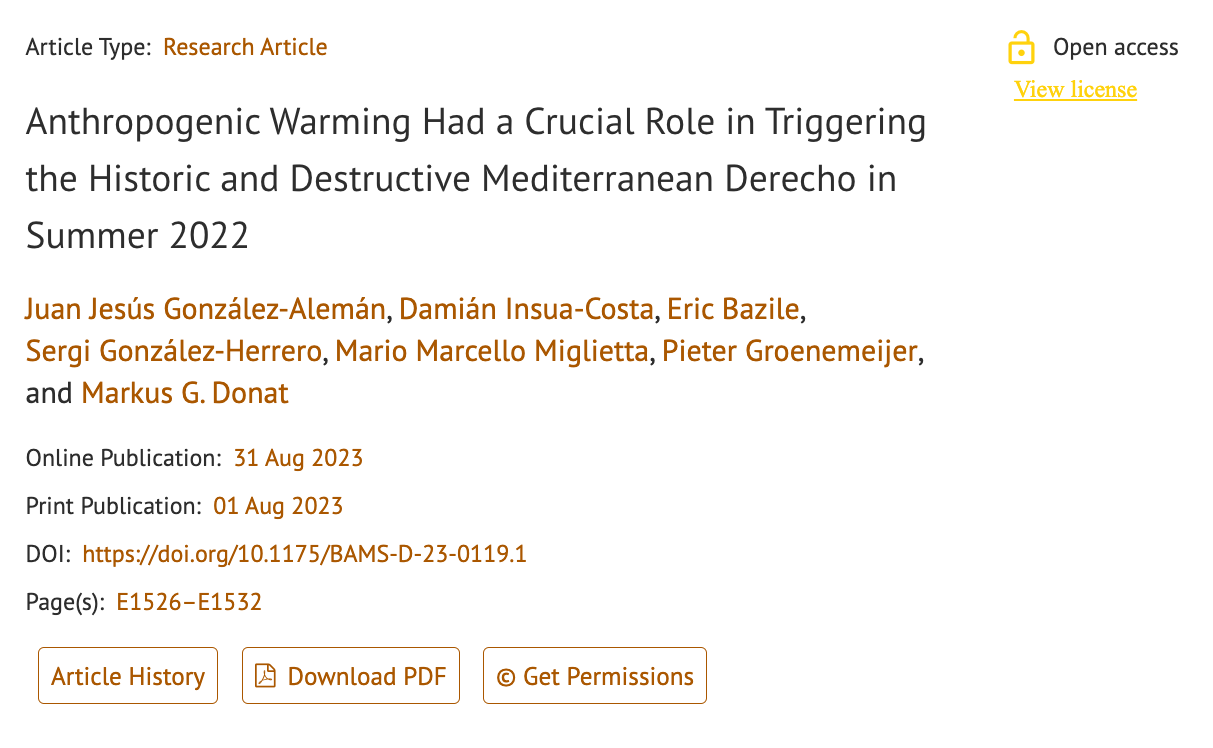
\includegraphics[width = \textwidth]{../img/derecho2022c}

\end{frame}
% ----------------------------------------------------

% ----------------------------------------------------
\begin{frame}
\frametitle{Empirical Research process}
\centering

\resizebox{\linewidth}{!}{
\begin{tikzpicture}
\node (topic) at (1,0) {Topic};
\node (rq) at (2.5,0) {RQ};
\node (theory) at (4,0) {Theory};
\node (measure) at (6,0) {Measure};
\node (strat) at (8,0) {Strategy};
\node (analyses) at (10,0) {Analyses};
\node (results) at (12,0) {Results};

\draw[->, line width=0.4mm] (topic) to[out=280, in=260] (rq) node[] {};
\draw[->, line width=0.4mm] (rq) to[out=280, in=260] (theory) node[] {};
\draw[->, line width=0.4mm] (theory) to[out=280, in=260] (measure) node[] {};
\draw[->, line width=0.4mm] (measure) to[out=280, in=260] (strat) node[] {};
\draw[->, line width=0.4mm] (strat) to[out=280, in=260] (analyses) node[] {};
\draw[->, line width=0.4mm] (analyses) to[out=280, in=260] (results) node[] {};
\draw[->, line width=0.4mm, red] (results) to[out=160, in=20] (topic) node[] {};

\end{tikzpicture}}

\end{frame}
% ----------------------------------------------------


% ----------------------------------------------------
\begin{frame}
\frametitle{Key ingredientes}
\centering

\begin{flushleft}
In every case, when we talk about \textit{quantitative empirical research}, we will work with \textbf{variation} across \textbf{observations} at a given \textbf{unit of analyses/observation}, from which we infer stuff
\end{flushleft}


\vspace{10pt}

\begin{itemize}[<+->]
  \item[1.] Observation
  \item[2.] Unit
  \item[3.] Variables
  \item[4.] Variation
\end{itemize}

\end{frame}
% ----------------------------------------------------

% ----------------------------------------------------
\begin{frame}
\frametitle{What's the unit of analyses in the data behind this graph?}
\centering

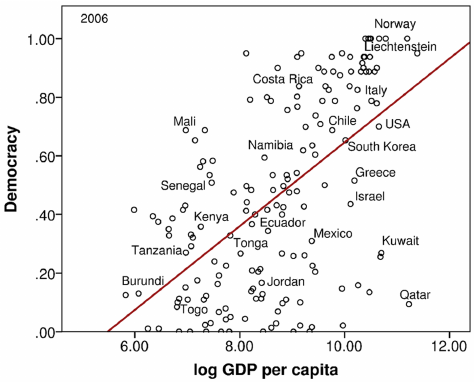
\includegraphics[width = 0.8\textwidth]{../img/ua1}

\end{frame}
% ----------------------------------------------------

% ----------------------------------------------------
\imageframe{../img/ua2}
% ----------------------------------------------------

% ----------------------------------------------------
\imageframe{../img/ua3}
% ----------------------------------------------------

% ----------------------------------------------------
\begin{frame}
\frametitle{Reading}
\centering

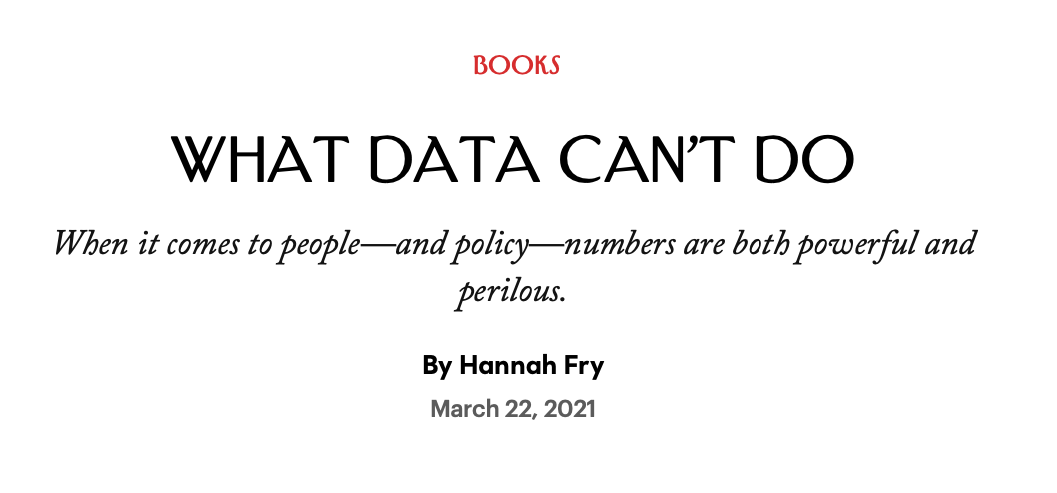
\includegraphics[width = 0.8\textwidth]{../img/reading}

\end{frame}
% ----------------------------------------------------

% ----------------------------------------------------
\begin{frame}
\frametitle{Research process in detail (1)}
\centering

\begin{itemize}
  \item[$>$] From \textbf{topic} (or problem) to the \BGyellow{\textbf{research question}}
  \item[]
  \item<2-> Difference between motivation and question
  \item<3-> What are good \& bad research questions?
  \begin{itemize}
    \item Answerable
    \item Relevant: importance and connection theory/empirics (*)
  \end{itemize}
  \item[]<4->
  \item[]<4-> Examples
  \begin{itemize}
    \item What is the best Netflix show?
    \item What can we do to help poor countries develop?
    \item What are the shopping patterns of the Spanish population?
    \item {\small (*) Do individuals from minorities support the use of violence?}
  \end{itemize}
\end{itemize}

\end{frame}
% ----------------------------------------------------

% ----------------------------------------------------
\begin{frame}
\frametitle{Research process in detail (2)}
\centering

\begin{itemize}
  \item[$>$] From \textbf{RQ} to \BGyellow{\textbf{theory}}
  \item[]
  \item<2-> What is a theory? Importance
  \item<3-> Arguments and mechanisms
  \item<3-> Micro-level, macro-level, and both
  \item<4-> Good theories or arguments
  \begin{itemize}
    \item Testable
    \item Credible
  \end{itemize}
\end{itemize}

\end{frame}
% ----------------------------------------------------

% ----------------------------------------------------
\begin{frame}
\frametitle{Research process in detail (3)}
\centering

\begin{itemize}
  \item[$>$] From \textbf{theory} to \BGyellow{\textbf{measurement}}
  \item[]
  \item Concepts
  \item Operationalization in variables
  \item Measurement
  \item Unit of analysis
\end{itemize}

\end{frame}
% ----------------------------------------------------

% ----------------------------------------------------
\begin{frame}
\frametitle{Research process in detail (4)}
\centering

\begin{itemize}
  \item[$>$] From \textbf{measurement} to \BGyellow{\textbf{strategy}}
  \item[]
  \item Once you have your variables measured, what variation are you going to look at?
  \begin{itemize}
    \item Think about how kids learn
  \end{itemize}
  \item Descriptive and causal inference
  \item (Experiments) (*)
\end{itemize}

\end{frame}
% ----------------------------------------------------

% ----------------------------------------------------
\begin{frame}
\frametitle{Research process in detail (5)}
\centering

\begin{itemize}
  \item[$>$] From \textbf{strategy} to \BGyellow{\textbf{analyses}}
  \item[]
  \item We're \textbf{not} covering this in this course
  \item This basically means choosing how you are going to analyze the variation you have
  \item Comparisons, models, statistics
  \item \textbf{Question:} what is the role of statistics in research design?
\end{itemize}

\end{frame}
% ----------------------------------------------------

% ----------------------------------------------------
\begin{frame}
\frametitle{Research process in detail (6)}
\centering

\begin{itemize}
  \item[$>$] From \textbf{analyses} to \textbf{results} and back to \BGyellow{\textbf{topic}}
  \item[]
  \item Interpretation
  \item Relevance
  \item \textbf{External validity}
\end{itemize}

\end{frame}
% ----------------------------------------------------

% ----------------------------------------------------
\begin{frame}
\frametitle{Simplyfing}
\centering

\begin{itemize}
  \item[1.] Formulate one (or more) RQ from a topic/problem
  \item[2.] Develop a theoretical argument related to that RQ
  \item[3.] Building on theory, think about what and how to measure
  \item[4.] What variation are you going to look at? (and what data analysis tools do you need?)
  \item[5.] What can you really learn from the results?
\end{itemize}

\end{frame}
% ----------------------------------------------------

% ----------------------------------------------------
\begin{frame}
\frametitle{Let's go through an example}
\centering

You are hired by the city government as a quantitative analyst to tackle the problem of \textbf{urban traffic in Madrid} and offer suggestions to improve it

\end{frame}
% ----------------------------------------------------

% ----------------------------------------------------
\begin{frame}
\frametitle{Course logistics}
\centering

\begin{itemize}
  \item Tuesdays 18:00--21:00 (most of the time)
  \item Seven sessions between September 12th and October 24th
  \item Room 2.A.04 (Puerta de Toledo)
  \item[]
  \item My email: \texttt{francisco.villamil@uc3m.es}
  \item Office hours
\end{itemize}

\end{frame}
% ----------------------------------------------------

% ----------------------------------------------------
\begin{frame}
\frametitle{Course logistics: evaluation}
\centering

\begin{itemize}
  \item Participation (10\%)
  \item Research papers reviews (15\%)
  \item Workshop group presentation (20\%)
  \item Workshop feedback (15\%)
  \item Final essay (40\%)
\end{itemize}

\end{frame}
% ----------------------------------------------------

% ----------------------------------------------------
\begin{frame}
\frametitle{Workshop and final essay}
\centering

\begin{itemize}
  \item In the workshop we will have around 12-15 slots (10 minute presentation \& 10 feedback) so we need to do \textbf{group presentations}
  \begin{itemize}
    \item We can adjust time once we know the final number of groups
  \end{itemize}
  \item I do not mind if you do the final essay individually or in groups (max 3/4)
  \item Two good options:
  \begin{itemize}
    \item Do a group presentation covering different strategies and individual essay with each of them
    \item Do a group final essay
  \end{itemize}
\end{itemize}

\end{frame}
% ----------------------------------------------------

% ----------------------------------------------------
\begin{frame}
\frametitle{Final essay}
\centering

\begin{itemize}
  \item Get a topic or problem and go through all the steps in the research process
  \item No need to do data analyses or statistics (but you could show something if it's relevant)
  \item \textbf{Most important thing}: show me you understand how you can learn something about the topic from quantiative data, what different strategies you could use and what are the general and specific limitations of them
  \item Word limit: \textbf{5000 words} (we can talk in case of group essays)
  \begin{itemize}
    \item Appendix obviously does not count
  \end{itemize}
  \item {\color{red}{Deadline}}: \textbf{November 5th, 23.59h} (exam week)
\end{itemize}

\end{frame}
% ----------------------------------------------------

% ----------------------------------------------------
\begin{frame}
\frametitle{Course logistics: calendar}
\centering

\begin{itemize}
  \item 4 lectures (including today)
  \begin{itemize}
    \item In sessions 2--4, we'll discuss a paper in the second half
    \item You have to submit some comments/critique (5\% each), \textbf{before} class (email or paper)
  \end{itemize}
  \item A workshop (double session)
  \item Final lecture on advanced topics, overview, and questions
\end{itemize}

\end{frame}
% ----------------------------------------------------

% ----------------------------------------------------
\begin{frame}
\frametitle{Course logistics: calendar}
\centering

\begin{itemize}
  \item Sept 12th: Introduction
  \item Sept 19th: Elements of quantitative data
  \item Sept 26th: Causality and experimental evidence
  \item Oct 3rd: Causal inference with observational data
  \item \asher{\textit{Oct 10th: no class}}
  \item Oct 17th (15h-21h): Workshop (double session)
  \item Oct 24th (15h-18h): Advanced topics and overview
\end{itemize}

\end{frame}
% ----------------------------------------------------

% ----------------------------------------------------
\begin{frame}
\frametitle{Your calendar in October}
\centering

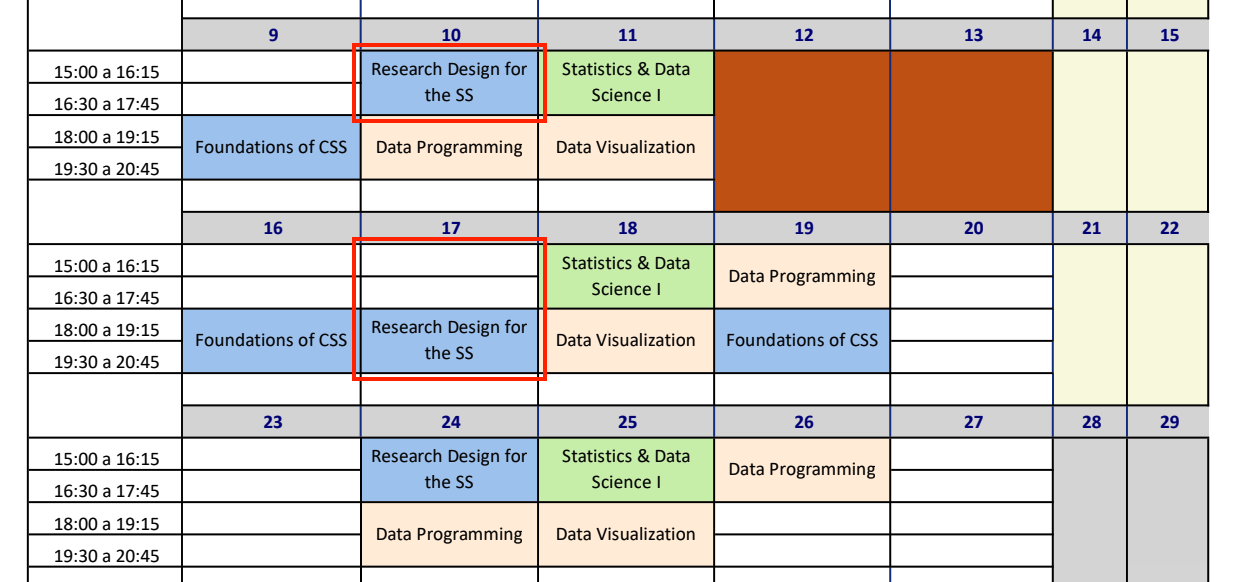
\includegraphics[width = \textwidth]{../img/calendar}

\end{frame}
% ----------------------------------------------------

% ----------------------------------------------------
\begin{frame}
\frametitle{Textbooks and resources}
\centering

\begin{itemize}
  \item \textbf{Nick Huntington-Klein, \href{https://theeffectbook.net/}{\textit{The Effect: An Introduction to Research Design and Causality}} (Chapman and Hall/CRC, 2021).}
  \item Kosuke Imai, \textit{Quantiative Social Science: An Introduction} (Princeton UP, 2017).
  \item Dimiter Toshkov, \textit{Research Design in Political Science} (Palgrave, 2016)
  \item Scott Cunningham, \href{https://mixtape.scunning.com/}{\textit{Causal Inference: The Mixtape}} (Yale University Press, 2021).
\end{itemize}

\end{frame}
% ----------------------------------------------------

% ----------------------------------------------------
\begin{frame}
\frametitle{Papers to read}
\centering

\begin{itemize}
  \item[1.] Carl Müller-Crepon, Philipp Hunziker, and Lars-Erik Cederman. \href{https://journals.sagepub.com/doi/10.1177/0022002720963674}{Roads to Rule, Roads to Rebel: Relational State Capacity and Conflict in Africa.} \textit{Journal of Conflict Resolution} 65(2--3): 563--590.
  \item[2.] Andrew M. Guess \textit{et al.} \href{https://www.science.org/doi/10.1126/science.abp9364}{How do social media feed algorithms affect attitudes and behavior in an election campaign?} \textit{Science} 381(6656): 398--404.
  \item[3.] TBD
\end{itemize}

\end{frame}
% ----------------------------------------------------

% ----------------------------------------------------
\begin{frame}
\frametitle{Next week's reading}
\centering

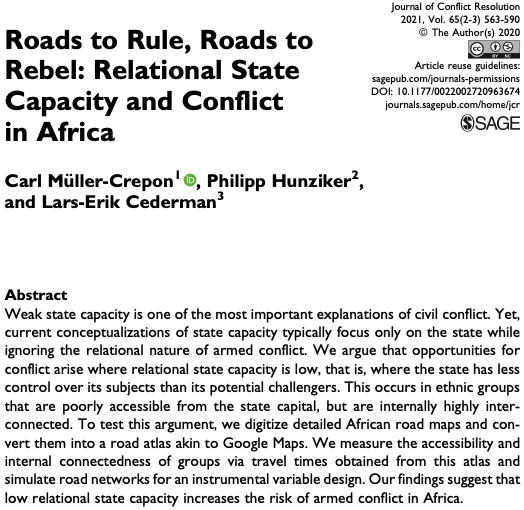
\includegraphics[width = 0.7\textwidth]{../img/mullercrepon}

\end{frame}
% ----------------------------------------------------

% ----------------------------------------------------
\begin{frame}
\frametitle{}
\centering

Questions?

\end{frame}
% ----------------------------------------------------

%\appendix
%\renewcommand{\theframenumber}{A\arabic{framenumber}}
%\renewcommand{\insertframenumber}{A\arabic{framenumber}}

% ====================================================
\end{document}
